\documentclass{pracamgr}
\usepackage{fontspec}
%\usepackage{microtype} % does not work with xetex older than 0.9997
\usepackage{polski}
\usepackage{polyglossia}
\usepackage[debugshow]{graphicx}

\setmainfont[Mapping=tex-text]{DejaVu Serif}
\newfontface\cyr{Hirmos Ponomar}
\newfontface\lat{DejaVu Serif}

\renewcommand{\chaptername}{Rozdział} % fix for ugly 'ł'

\author{Mikołaj Dądela}
\nralbumu{262484}

\title{Corthus -- korpus równoległy z interfejsem internetowym i
  przeszukiwarką fonetyczną}
\tytulang{Corthus -- a parallel corpus with internet interface and a
  phonetic search engine}

\kierunek{Informatyka}
\opiekun{dra hab. Adama Przepiórkowskiego\\ Instytut Informatyki}
\date{Wrzesień 2012}

\dziedzina{11.3 Informatyka} % wg klasyfikacji Socrates-Erasmus
\klasyfikacja{ H. Information Systems \\
               H.3 Information Storage and Retreival \\
               H.3.1 Content Analysis and Indexing } % wg ACM

\keywords{tłumaczenie, alignment, teksty równoległe, wyszukiwanie
  fonetyczne, metaphone, Python}

\begin{document}
\maketitle

\begin{abstract}
  W swojej pracy stworzyłem korpus równoległy z tekstów liturgicznych
  używanych przez Cerkiew Prawosławną w językach polskim,
  cerkiewno\-{}słowiańskim i staro\-{}greckim. Korpus można przeglądać i
  przeszukiwać poprzez dwa interfejsy: wiersza poleceń oraz
  internetowy. Przeszukiwanie opiera się na przybliżonej wymowie słów,
  aby można było było znaleźć słowo, którego zna się tylko wymowę.
\end{abstract}

\tableofcontents
%\listoffigures
%\listoftables

%%%%%%%%%%%%%%%%%%%%%%%%%%%%%%%%%%%%%%%%%%%%%%%%%%%%%%%%%%%%%%%%%%%%%%

\chapter{Wprowadzenie}
\addcontentsline{toc}{chapter}{Wprowadzenie}

W swojej pracy stworzyłem korpus równoległy z tekstów liturgicznych
używanych przez Cerkiew Prawosławną w językach polskim,
cerkiewno\-{}słowiańskim i staro\-{}greckim. Korpus można przeglądać i
przeszukiwać poprzez dwa interfejsy: wiersza poleceń oraz
internetowy. Przeszukiwanie opiera się na przybliżonej wymowie słów,
aby można było było znaleźć słowo, którego zna się tylko wymowę.

\section{Cel}\label{cel}

Głównym celem mojej pracy było ułatwienie szerszej publiczności
dostępu do tekstów liturgicznych w różnych językach i sprawienie, żeby
były zrozumiałe dzięki możliwości równoległego ich czytania i łatwo
dostępne dzięki wyszukiwarce.

Pragnąłem również ułatwić zainteresowanym naukę języka
cerkiewno\-{}słowiańskiego, poczynając już od pierwszego jej etapu, którym
jest nauka czytania. Chciałem również poprzez zestawienie tekstów
unaocznić analogiczny, a często identyczny szyk zdań w językach
starogreckim i cerkiewno\-{}słowiańskim.

Trwa obecnie dyskusja na temat zasadności tłumaczenia tekstów
liturgicznych na język polski i poprawności istniejących tłumaczeń --
chciałem więc stworzyć pomoc do ich badania, jak również do
potencjalnego tłumaczenia kolejnych podobnych tekstów na język
polski.

\section{Wizja}\label{wizja}

Planowałem stworzyć serwis internetowy, w którym można łatwo
przeglądać, przeszukiwać i porównywać teksty w różnych językach, w
pisowni oryginalnej lub w transkrypcji fonetycznej na język polski.

Ważnym elementem projektowanego serwisu była przeszukiwarka
wspomnianych tekstów. Głównym jej celem była nie tyle precyzja
wyszukiwania, co łatwość jej użycia, gdyż pisownia cerkiewno\-{}słowiańska
i starogrecka jest na tyle skomplikowana, że nie można założyć, że
użytkownik bezbłędnie wpisze w wyszukiwarkę frazę z szukanego tekstu.

Ciekawą możliwością dalszego rozwinięcia projektu byłaby implementacja
rytmu kalendarza prawosławnego i udostępnienie linku „tekst na
dzisiaj".

Główne cele użycia serwisu byłyby takie, jak wymieniłem w rozdziale
\ref{cel} -- starałem się jednak stworzyć na tyle ogólną
implementację, żeby można było jej później użyć do innych zastosowań,
np. stworzenia bazy tłumaczeń tekstów technicznych. Niektóre algorytmy
w sposób nieunikniony używają różnych wersji dla trzech języków, z
których składała się moja baza, ale nic nie stoi na przeszkodzie, żeby
dodać analogiczne funkcje do obsługi innych języków.

%%%%%%%%%%%%%%%%%%%%%%%%%%%%%%%%%%%%%%%%%%%%%%%%%%%%%%%%%%%%%%%%%%%%%%

\chapter{Przygotowania i eksperymenty}

Zacząłem swoją pracę od poszukiwań gotowych narzędzi, które
odpowiadałoby przynajmniej części założeń opisanych powyżej. Postaram
się tu krótko opisać swoje doświadczenia z nimi.

\section{Hunalign}

Hunalign jest narzędziem zestawiającym 2 teksty na poziomie zdań
(zakładając, że są już podzielone na zdania), bazując na ich
długościach i (opcjonalnie) na słowniku. Jeśli jednak nie dysponujemy
słownikiem, można uruchomić Hunaligna z opcją {\tt -realign} --
Hunalign wówczas po pierwsym, wstępnym dopasowaniu próbuje wygenerować
przybliżony słownik, a następnie dopasowuje teksty ponownie z użyciem
tego słownika. Dopasowania generowane przez Hunaligna są niemal w
100\% poprawne, jeśli teksty dokładnie sobie odpowiadają. Niestety
teksty, z którymi pracowałem, bardzo często różniły się od siebie
dużymi fragmentami tekstu, co powodowało przesunięcia w dopasowaniu.

Mimo to Hunalign okazał się bardzo przydatny, gdyż, bazując głównie na
długości zdań, generuje dopasowanie, które może zostać wykorzystane do
wygenerowania przybliżonego słownika fraz, który następnie może
posłużyć do polepszenia dopasowania.

\section{GIZA++}

GIZA++ \cite{giza} jest narzędziem tworzącym dopasowanie na poziomie
słów z już dopasowanych par zdań. Nie użyłem jej w mojej pracy,
ponieważ przede wszystkim potrzebowałem dopasowania na poziomie
zdań. Dopasowanie na poziomie słów jest jednak poza zakresem
niniejszej pracy (chociaż byłoby niewątpliwie ciekawym i użytecznym
rozszerzeniem tej pracy).

\section{Poliqarp}

Poliqarp \cite{poliqarp} jest darmowym (swobodnym) zestawem narzędzi
do przeszukiwania dużych korpusów. Wspiera obsługę korpusów
otagowanych znacznikami morfosyntaktycznymi i pozwala na
przeszukiwanie korpusu za pomocą złożonych zapytań. Jednak teksty,
którymi się zajmowałem w swojej pracy, nie były otagowane, więc nie
mógłbym też wykorzystać pełni możliwości Poliqarpa. Poliqarp nie
posiada również obsługi korpusów równoległych.

\section{Wzorce odmiany i lematyzacja}

Próbowałem uprościć Hunalignowi generowanie przybliżonego słownika
poprzez usunięcie końcówek morfosyntaktycznych ze słów. Nie znalazłem
jednak gotowej biblioteki, wykonującej takie zadanie. Rozważałem
ręczną implementację tej funkcjonalności, ale po przyjrzeniu się
wzorcom odmiany języka cerkiewno\-{}słowiańskiego \cite{strach}
zrezygnowałem. Początkowo przybliżałem lematyzację skracaniem słowa do
5 liter, a po implementacji Metaphone zauważyłem, że Metaphone również
łączy pod wspólnym kluczem wiele form fleksyjnych jednego słowa, więc
w końcowej wersji projektu dopasowuję do siebie nie oryginalne teksty,
lecz ciągi kluczy Metaphone z nich utworzone.

\section{Słowniki}

Szukałem również słownika cerkiewno\-{}słowiańsko-polskiego, lecz
znalazłem tylko jeden \cite{znosko}, autorstwa O. Aleksego Znosko, i
nie udało mi się go zdobyć w wersji cyfrowej -- na mail do wydawcy
otrzymałem odpowiedź, że autor zmarł przed wydaniem tego słownika, i
plik z zawartością słownika nigdzie się nie zachował.

%%%%%%%%%%%%%%%%%%%%%%%%%%%%%%%%%%%%%%%%%%%%%%%%%%%%%%%%%%%%%%%%%%%%%%

\chapter{Architektura projektu}

Cała implementacja została napisana w języku Python.

\section{Katalog \textit{toolkit} -- główna funkcjonalność}

TODO

toolkit/translit

Wiele skryptów z tego folderu można wywołać z linni komend, aby
wykonać różne zadania (patrz rozdział \ref{r:cli}).

\section{Katalog \textit{www} -- interfejs internetowy}

Interfejs internetowy został szczegółowo opisany w rozdziale
\ref{r:www}.

\section{Katalog \textit{texts} -- baza tekstów}

Katalog \textit{texts} zawiera wszystkie teksty.

Moja decyzja o używaniu plików tekstowych zamiast bazy danych była
powodowana prostotą operacji na plikach w konsoli, i możliwością
łatwej zmiany w organizacji tekstów. Łatwość zmian była dla mnie
bardzo ważna, bo w początkowej fazie rozwoju projektu nie było jasne,
w jaki sposób system będzie korzystał z tekstów.

Nazwa pliku z tekstem źródłowym ma postać
{\tt texts/}\textit{książka}{\tt /}\textit{rozdział}{\tt /}\textit{język}{\tt .txt}
, gdzie \textit{język} jest jednym spośród ``pl'', ``cu''
\footnote{``cu'' oznacza język cerkiewnosłowiański, zgodnie ze standardem ISO 639-1.}
 i ``el''.

\section{Katalog \textit{external} -- zewnętrzne biblioteki i narzędzia}

Katalog \textit{external} zawiera zewnętrzne biblioteki, z których
korzysta projekt. Na chwilę obecną są to Hunalign \cite {hunalign} i
Whoosh \cite {Whoosh}.

%%%%%%%%%%%%%%%%%%%%%%%%%%%%%%%%%%%%%%%%%%%%%%%%%%%%%%%%%%%%%%%%%%%%%%

\chapter{Przygotowanie danych}

\section{Konwersja danych wejściowych}

Teksty pobrałem ze stron \cite{orthlib}, \cite{analogion} i
\cite{liturgia}. Pliki z tych stron były odpowiednio w formatach
HIP \footnote{HIP -- standard zapisu tekstu
  cerkiewno\-{}słowiańskiego. Więcej szczegółów w dodatku \ref{encoding}} ,
HTML i DOC.

Zdecydowałem wszystkie te pliki przekonwertować do zwykłego tekstu
kodowanego w UTF-8. Napisałem w tym celu skrypt w Pythonie, który
korzystał dodatkowo z Elinksa i AbiWorda. Zdecydowałem się na
kodowanie UTF-8, bo dzięki niemu mogłem używać jednego kodowania dla
wszystkich plików, i uznałem, że to uproszczenie rekompensuje 2 razy
większy rozmiar pliku. Decyzja o przejściu na zwykły tekst oznaczała
również rezygnację z formatowania. Połamałem akapity na linie nie
dłuższe niż 70 znaków, rozdzielając je pustymi liniami (tak jak w
TeXu), tak żeby można było je wygodnie przeglądać w dowolnym edytorze
tekstu lub w konsoli.

\section{Dopasowywanie tekstów}

Na początku potrzebne było dopasowanie tekstów na poziomie plików. Nie
było to trywialne, bo teksty były różnie zredagowane, i bardzo często
jeden plik odpowiadał kilku plikom w innym języku. Wykonałem to
zadanie ręcznie, z pomocą prostego skryptu dzielącego plik na części w
odpowiednich miejscach.

%Teksty są w trzech językach, więc „normalne" dopasowanie dwóch języków
%by nie wystarczyło.

%\section{Modele tłumaczenia}

%Próbowałem różnych modeli.

%Trigram→trigram wygląda nieźle, bo jest sporo powtarzających się trigramów -- ciężko sprawdzić, czy są tłumaczone tak samo

%Akapit→akapit wygląda bardzo obiecująco, bo powtarzających się akapitów jest sporo, i w tłumaczeniu powinno to wychodzić podobnie. Może można założyć, że jeśli akapit X został przetłumaczony na Y, to każde inne wystąpienie X będzie też tłumaczone na Y?

Stworzyłem wstępne dopasowania Hunalignem.

Z nich wydorębniłem pary tłumaczeń, które się powtarzały (bardzo duża
poprawność dopasowań na tych parach!!!).

Następnie sprawdziłem, ile procent zdań stanowią te, które udało się w
ten sposób sparować. Okazało się, że to ok. 20\%!

TODO: ALGORYTM alignera!!! (i może wykresy)

TODO: Dopasowanie 3 języków!

TODO: WYNIKI!!! ewaluacja!!!

\section{Transformacje tekstu (pakiet {\tt translit})}

Aby poprawnie wyświetlić tekst w języku cerkiewno\-{}słowiańskim,
potrzebna była specjalna czcionka, która oprócz liter zawierała
również zestaw ligatur, potrzebnych do poprawnego ułożenia znaków
diakrytycznych nad konkretnymi literami. Przygotowanie tekstu do
wyświetlenia w takiej czcionce również wymagało napisania prostego
skryptu.

Język cerkiewno\-{}słowiański w zapisie często występujących słów korzysta
ze skrótów. Polegają one zazwyczaj na opuszczeniu samogłosek
(zazwyczaj tytło proste, {\cyr\ ҃}) lub środkowej części wyrazu
(zazwyczaj tytła literowe, {\cyr ⷭ\ \ ⷢ\ \ ⷣ}). Język
cerkiewno\-{}słowiański korzysta ponadto z własnego systemu zapisu
liczb. Wobec tego, aby dokonać transkrypcji fonetycznej takiego
tekstu, należało najpierw rozwinąć wszystkie skróty i zamienić liczby
na cyfry arabskie. Napisałem w tym celu moduł {\tt translit.expand\_cu},
zawierający listę 130 różnych skrótów i obsługujący liczby do 10
tysięcy (większe liczby nie występują w tekstach). Aby konwersja mogła
działać wydajnie, skompilowałem wszystkie wzorce skrótów do jednego
wyrażenia regularnego.

Następnie zaimplementowałem transkrypcję fonetyczną na polski w module
{\tt cu2pl}. Największy problem sprawiło mi tutaj dostosowanie wyniku
do polskiej pisowni (przede wszystkim chodziło tu o litery „i" i „j" w
różnych kontekstach).

Zaimplementowałem również transkrypcję fonetyczną z języka
starogreckiego na polski. Dokonuję tej transkrypcji jednak zgodnie z
regułami wymowy współczesnej Greki, dlatego, że w ten sposób są zwykle
czytane. Konwersja zachodzi w dwóch etapach: najpierw upraszczam
zapis, usuwając znaki przydechu (dasia, prosgegrammeni, ypogegrammeni)
i zamieniając wszystkie rodzaje akcentu (tonos, oxia, varia,
perispomeni) na jeden (tonos), i dopiero wtedy dokonuję zamiany
greckich liter i dyftongów na polskie odpowiedniki
fonetyczne. Pierwszy etap konwersji wykonuje moduł {\tt
  translit.simplify\_el}, a drugi {\tt translit.el2pl}.

\section{Metaphone}

Do rozmytego wyszukiwania według wymowy słów potrzebowałem algorytmu,
działającego podobnie do Soundex [ref], generującego dla słów klucze
odpowiadające przybliżonej wymowie. Z jednej strony Soundex był do
tego celu zbyt mało dokładny, z drugiej strony transkrypcja fonetyczna
wszystkich tekstów na polski nie pozwoliłaby na znalezienie słowa,
jeśli zostało błędnie wpisane w wyszukiwarkę.

Zainspirował mnie algotytm Metaphone [ref]. Nie zastosowałem jednak
dokładnie tego algorytmu, lecz stworzyłem jego wersję dostosowaną do
moich danych\footnote{W dalszej części pracy nazywam tę wersję po
  prostu ``metaphone''}. Działanie algorytmu dla danego słowa
przedstawia się następująco:

\begin{enumerate}
\item Jeśli dane słowo jest liczbą, zwróć tę liczbę dodając ``\#'' na
  początku.
\item Jeśli język nie został podany, wykryj język tekstu. Jeśli tekst
  zawiera znaki, których nie udało się rozpoznać, zwróć ``?''.
\item Użyj tablicy podstawień dla danego języka (patrz tabela
  \ref{tab:metaphone}). Uproszczona wersja tej tablicy znajduje się
  poniżej. W języku cerkiewno\-{}słowiańskim dodatkowo następuje tu
  rozwijanie skrótów i konwersja liczb. Jeśli okazało się, że mieliśmy
  do czynienia z liczbą, zwracamy jej wartość poprzedzoną znakiem
  ``\#''.
\item Usuń wszystkie samogłoski, zaczynając od drugiej litery
  wynikowego ciągu znaków.
\end{enumerate}

\begin{table}
  \caption{Uproszczona tablica podstawień dla mojej wersji algorytmu
    Metaphone}
  \renewcommand{\arraystretch}{1.2}
  \begin{tabular}{|l|l|l|l|}
    \hline
    metaphone & pl           & cu       & el      \\
    \hline
    a         & a            & \cyr{а          } & α       \\
    e         & e, ę         & \cyr{е, э, ѣ    } & ε, αι   \\
    i         & i, y         & \cyr{ѵ̀, и, ы, і} & ι, η, υ \\
    o         & o, ą         & \cyr{ѡ, о       } & ο, ω    \\
    u         & u, ó         & \cyr{у, ѹ       } & ου      \\
    \hline
    b         & b            & \cyr{б          } & μπ      \\
    c         & c, ć, cz     & \cyr{ц, ч, щ    } & τσ      \\
    d         & d, dz, dż    & \cyr{д          } & δ       \\
    f         & f            & \cyr{ф, ѳ       } & φ, θ    \\
    h         & g, h, ch     & \cyr{г, х       } & γ, χ    \\
    j         & j            & \cyr{й          } &         \\
    k         & k            & \cyr{к          } & κ       \\
    l         & l            & \cyr{ль         } & λ       \\
    7         & ł            & \cyr{л          } &         \\
    m         & m            & \cyr{м          } & μ       \\
    n         & n, ń         & \cyr{н          } & ν       \\
    p         & p            & \cyr{п          } & π       \\
    r         & r            & \cyr{р          } & ρ       \\
    s         & s            & \cyr{с          } & σ, ς    \\
    t         & t            & \cyr{т          } & τ       \\
    v         & w            & \cyr{в, ѵ       } & β, υ    \\
    z         & z, ź         & \cyr{з, ѕ       } & ζ       \\
    2         & ż, rz, sz, ś & \cyr{ж, ш       } &         \\
    \hline
  \end{tabular}
  \label{tab:metaphone}
\end{table}

\section{Wyszukiwarka}

Lucene, szuka po kluczach

%%%%%%%%%%%%%%%%%%%%%%%%%%%%%%%%%%%%%%%%%%%%%%%%%%%%%%%%%%%%%%%%%%%%%%

\chapter{Interfejs wiersza poleceń}\label{r:cli}

Większość modułów pakietu {\tt toolkit} udostępnia swoją
funkcjonalność poprzez prosty interfejs linii komend.

\section{{\tt fetcher}}

Fetcher pobiera odpowiedni tekst lub dopasowanie tekstów i wypisuje go
(w ładnie sformatowanej postaci) na standardowe wyjście.

\section{{\tt search}}

Skrypt przeszukuje bazę tekstów i wyświetla wynik. Wywołanie go z
opcją {\tt --create-index} powoduje utworzenie indeksu potrzebneg do
realizacji wyszukiwania. Wyszukiwarka opiera się na pakiecie Whoosh
\cite{whoosh}.

\section{{\tt aligner}}

TODO!

\section{{\tt Alignment}}

Skrypt Alignment.py zawiera klasę obsługującą dopasowania wielu
tekstów. Wywołany samodzielnie z wiersza poleceń, wyświetla podany
plik dopasowania.

Przykład użycia: \\
{\tt ./toolkit/Alignment.py test\_data/kanon\_izr.pl-cu.golden}

Fragment przykładowego wyniku działania skryptu można zobaczyć na
rysunku \ref{f:alignment}.

\begin{figure}[h]
  \caption{Przykładowe dopasowanie tekstów wyświetlone w konsoli.}
  \centering
    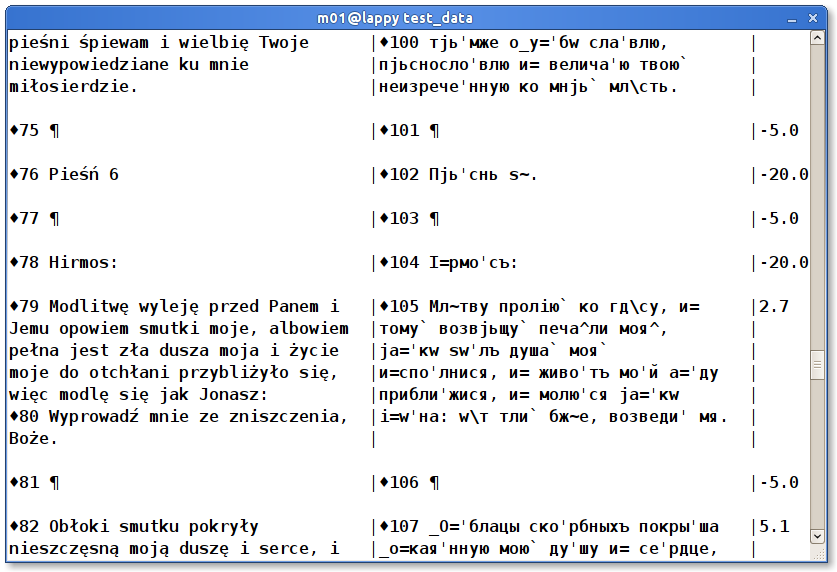
\includegraphics[width=5in]{console-alignment.png}
    \label{f:alignment}
\end{figure}

\section{Skrypty z pakietu {\tt translit}}

Wszystkie skrypty z pakietu {\tt translit} można uruchomić z linii
poleceń, aby dokonać odpowiednią transliterację na wybranym
tekście. Jako argument należy podać plik z tekstem, lub {\tt -}, aby
korzystać ze standardowego wejścia.

\begin{itemize}
\item {\tt expand\_cu.py} -- rozwijanie skrótów języka
  cerkiewno\-{}słowiańskiego i konwersja liczb na cyfry arabskie,
\item {\tt cu2pl.py} -- transkrypcja fonetyczna języka
  cerkiewno\-{}słowiańskiego na polski,
\item {\tt render\_cu.py} -- konwersja tekstu
  cerkiewno\-{}słowiańskiego do formatu UCS (patrz dodatek
  \ref{encoding}),
\item {\tt simplify\_el.py} -- ujednolicanie greckich akcentów i
  usuwanie innych znaków diakrytycznych,
\item {\tt el2pl.py} -- transkrypcja fonetyczna z (``uproszczonego'')
  greckiego na polski,
\item {\tt metaphone.py} -- zamiana tekstu na ciąg kluczy Metaphone.
\end{itemize}

%%%%%%%%%%%%%%%%%%%%%%%%%%%%%%%%%%%%%%%%%%%%%%%%%%%%%%%%%%%%%%%%%%%%%%

\chapter{Interfejs internetowy}\label{r:www}

Do utworzenia interfejsu internetowego użyłem frameworka Django
\cite{django}. Zdecydowałem się na ten wybór, ponieważ cały kod mojego
projektu został napisany w Pythonie, a Django jest najpopularniejszym
frameworkiem do tworzenia aplikacji internetowych w Pythonie, i miałem
z nim styczność podczas zajęć na MIM UW.

Interfejs internetowy można uruchomić do przetestowania wpisując
polecenie {\tt ./www/manage.py runserver} w terminalu w głównym
katalogu projektu. Powoduje to uruchomienie serwera HTTP, który
odpowiada na zapytania pod adresem {\tt http://127.0.0.1:8000/}.

Wygląd przykładowej strony można zobaczyć na rys. \ref{f:web2}.

\begin{figure}[h]
  \caption{Widok tekstu w interfejsie internetowym.}
  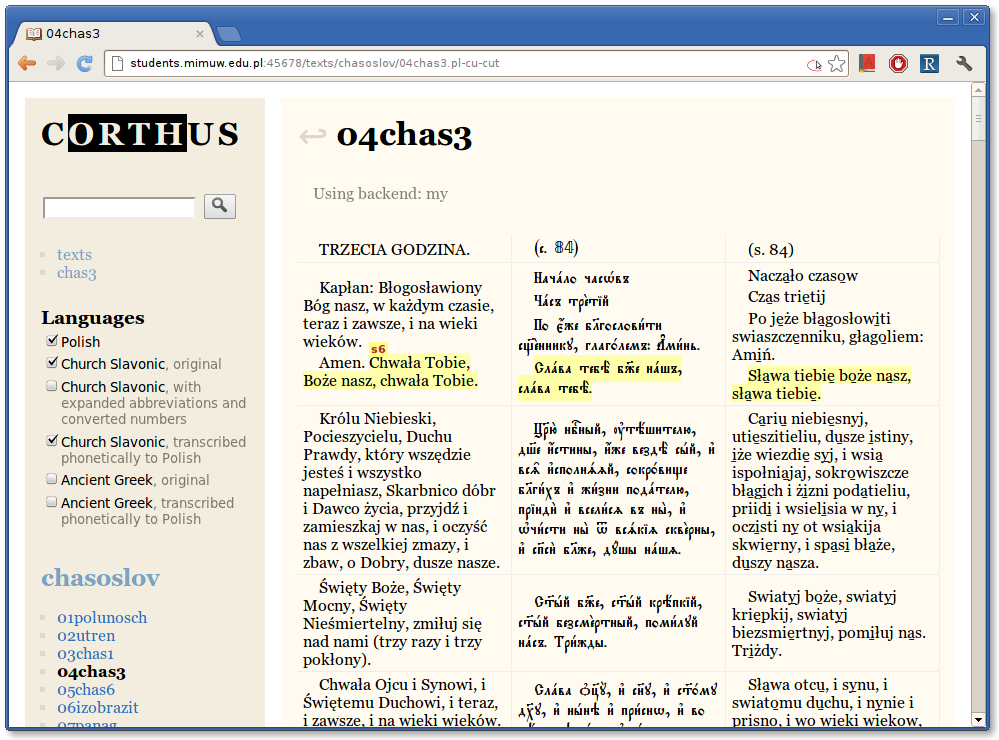
\includegraphics[width=\textwidth]{web2.png}
  \label{f:web2}
\end{figure}

\section{Model}

Model danych i operacje na nich obsługuje napisany przeze mnie pakiet
{\tt toolkit}. Nie potrzebowałem używać baz danych, które zwykle są
pomocne w podobnych projektach.

\section{Widoki}

Cały serwis internetowy obsługują 4 widoki.

\paragraph{Widok główny}
- strona główna, TODO!

\paragraph{Widok folderu}
Wyświetla spis treści książki lub spis książek.  To zadanie sprowadza
się do wyświetlenia odpowiednio sformatowanej listy plików.

\paragraph{Widok tekstu}
Wyświetla tekst równoległy. Po lewej stronie znajdują się pola wyboru
języków, których zmiana powoduje przeładowanie strony z nowymi
ustawieniami.

\paragraph{Widok wyników wyszukiwania}

\section{Szablony}

Szablony są prostymi plikami HTML, korzystającymi z zewnętrznych
arkuszy stylów CSS i skryptów w JavaScripcie.

Aby umożliwić przeglądanie tekstów cerkiewno\-{}słowiańskich osobom,
które nie mają zainstalowanej w systemie odpowiedniej czcionki, użyłem
deklaracji {\tt @font-face} z języka opisu formy prezentacji stron WWW
CSS. Deklaracja ta wprowadzona została dopiero w wersji 3 standardu,
dlatego może nie działać w starszych przeglądarkach. Jednak nowe
wersje wszystkich wiodących przeglądarek (Seamonkey 2.7.2, Opera
10.60, Firefox 3.6, Safari 4.0, Internet Explorer 9) obsługują ją
poprawnie. Starsze wersje Internet Explorera wyświetlają odstępy pod
znakami diakrytycznymi, jednak zawsze można ten problem obejść,
wyświetlając tekst w transkrypcji fonetycznej.

Zmiana języków jest obsługiwana przez krótki skrypt w języku
JavaScript. Preferencje użytkownika są zapisywane w pliku cookie, i
odczytywane przy następnej wizycie.

Podświetlanie odpowiadających sobie fragmentów tekstu jest również
obsługiwane przez skrypt JavaScript.

%%%%%%%%%%%%%%%%%%%%%%%%%%%%%%%%%%%%%%%%%%%%%%%%%%%%%%%%%%%%%%%%%%%%%%

\appendix
\chapter{Formaty plików}

\section{HIP i UCS -- tekst cerkiewno\-{}słowiański}
\label{encoding}

W czasach, kiedy więszość tekstów cerkiewno\-{}słowiańskich została
zdigitalizowanych, standard Unicode nie zawierał wszystkich znaków
potrzebych do zapisu tekstu w języku cerkiewno\-{}słowiańskim. W
odpowiedzi na to powstał standard HIP (opisany dokładnie w internecie
na stronie \cite{hip}). Pliki HIP to pliki tekstowe kodowane w
Windows-1251, używające cyrylicy wraz z niektórymi literami
łacińskimi, aby w ten sposób wyrazić wszystkie litery alfabetu
cerkiewno\-{}słowiańskiego. Zapis poszczególnych liter alfabetu (różne
warianty zapisu) zostały przedstawione w tabeli \ref{tab:hip}.

\begin{table}[ht!]
  \caption{Kodowanie znaków cerkiewno\-{}słowiańskich w standardzie HIP}
  \centering
    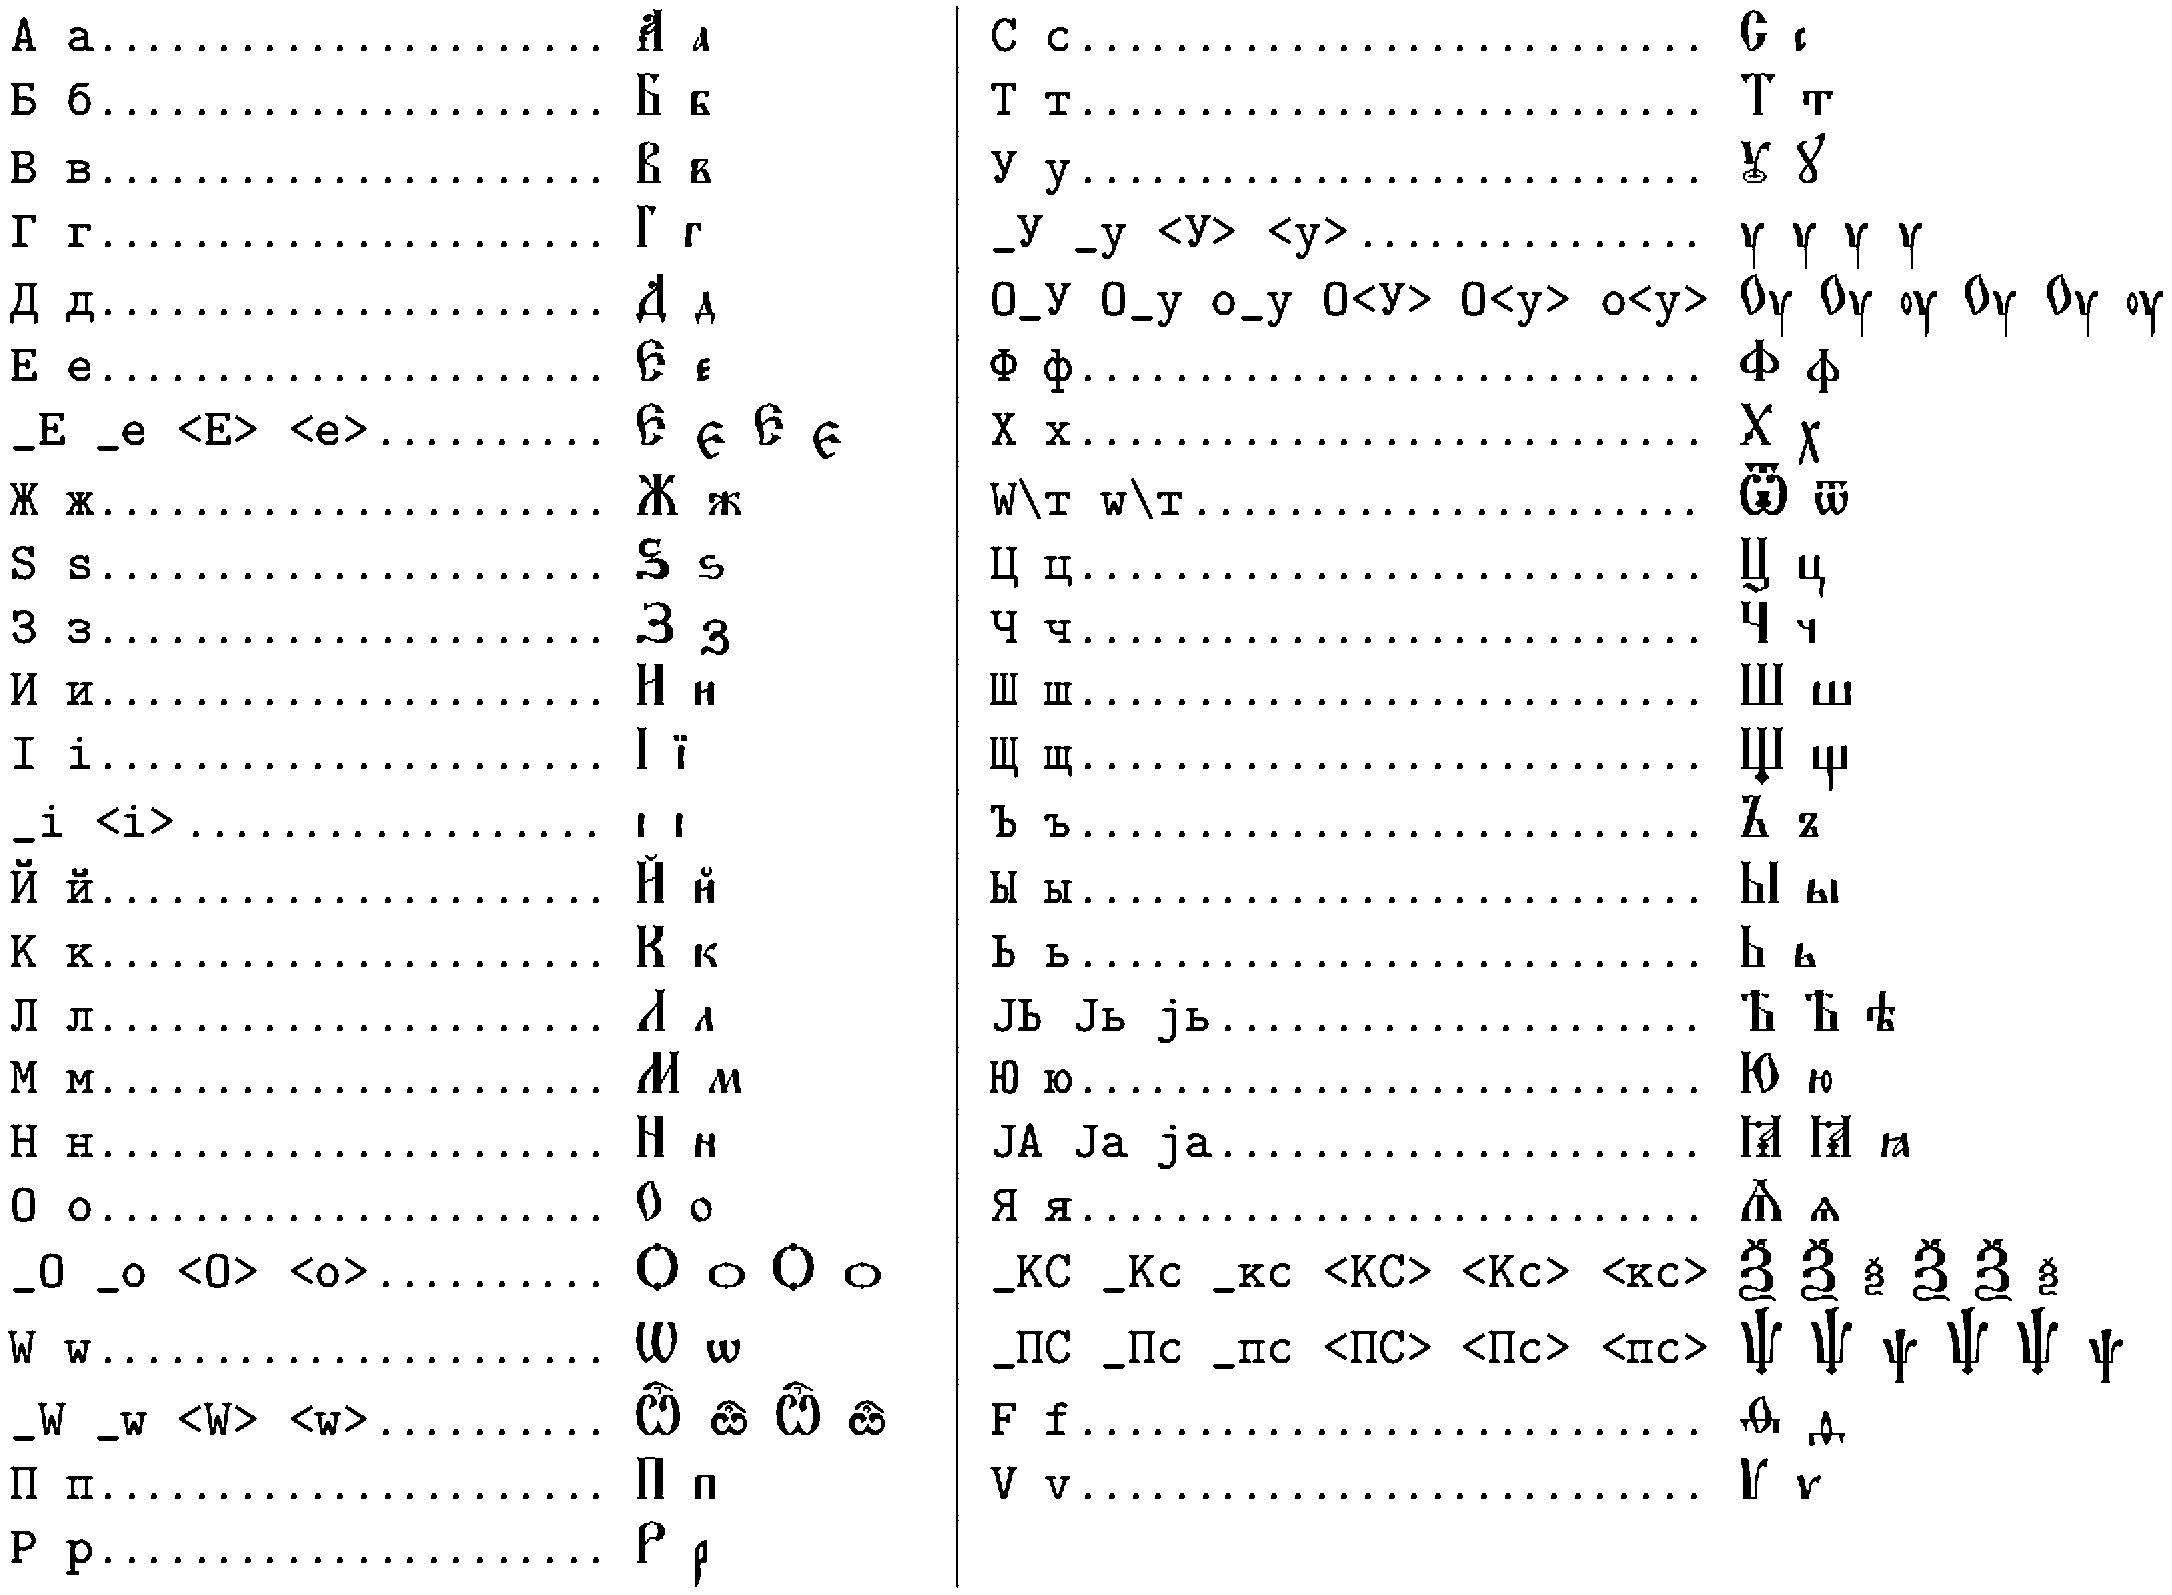
\includegraphics[width=\textwidth]{HIP-tabelka.png}
    \label{tab:hip}
\end{table}

Brakujące znaki były stopniowo dodawane do Unicode w wersjach 5.0.0
(2006), 5.1.0 (2008) i 5.2.0 (2009). Można więc obecnie zapisać tekst
cerkiewno\-{}słowiański w Unicode -- głównym problemem jest jednak
dostępność czcionek: czcionki obsługujące tytła literowe (znaki {\tt
  2DE0-2DFF}) i literę {\cyr ꙋ} ({\tt A64B}) są wielką rzadkością. Na
chwilę obecną udało mi się w internecie znaleźć tylko jedną czcionkę
obsługującą w pełni język cerkiewno\-{}słowiański, oznaczoną jako
``wersja beta'' \cite{ponomar}. Używam wobec tego starszych czcionek,
dostosowanych do kodowania UCS. Kodowanie UCS jest oparte na
Windows-1251. Znaki cyrylicy są w nim kodowane tak samo, jednak
wszystkie pozostałe pozycje strony kodowej są zajęte przez pozostałe
znaki języka cerkiewno\-{}słowiańskiego oraz ligatury tych znaków z
tytłami lub znakami diakrytycznymi (tylko w zestawieniach, gdzie takie
ligatury są potrzebne).

Dużą wadą takiego kodowania jest to, że jest ono niekompatybilne z
ASCII, i tak zakodowany tekst jest czytelny tylko jeśli zostanie
wyświetlony odpowiednią czcionką. Przykładowe czcionki dla tego
kodowania można pobrać ze strony \textit{Irmologion}
\cite{irmologion}.

\section{TXT -- pliki tekstowe}

Wszystkie pliki TXT w projekcie są kodowane w UTF-8. Zdecydowałem
jednak nie konwertować tekstów cerkiewno\-{}słowiańskich z zapisu HIP na
znaki odpowiadające im wedug standardu Unicode, ze względu na problemy
z wyświetlaniem tych znaków (patrz sekcja \ref{encoding}). Ta decyzja
pozwoliła mi na duże uproszczenie logiki programu, bo mogłem bardzo
łatwo przeglądać te pliki i wprowadzać w nich zmiany. Wadami tego
rozwiązania była konieczność rezygnacji z formatowania i nieco większy
rozmiar plików.

Połamałem akapity na linie nie dłuższe niż 70 znaków, rozdzielając
akapity od siebie pustymi liniami (analogicznie do TeXa), tak żeby można
było je wygodnie przeglądać w dowolnym edytorze tekstu lub w konsoli.

\section{Pliki dopasowań}

Dopasowania tekstów są zapisywane w formacie CSV, z tabulatorem
pełniącym rolę separatora pól. Jest to dokładnie taki format, jaki
zwraca Hunalign.

Nazwy plików dopasowań kończą się rozszerzeniem {\tt .hunalign}, {\tt
  .my} lub {\tt .golden}, w zależności od swojego pochodzenia. Kolejne
rozszerzenia oznaczają odpowiednio pliki wygenerowane przez Hunaligna,
pliki utworzone przez aligner z projektu i pliki dopasowań utworzone
ręcznie.

%%%%%%%%%%%%%%%%%%%%%%%%%%%%%%%%%%%%%%%%%%%%%%%%%%%%%%%%%%%%%%%%%%%%%%

\begin{thebibliography}{99}
\addcontentsline{toc}{chapter}{Bibliografia}

\bibitem{orthlib} Teksty cerkiewno\-{}słowiańskie:\\
  {\tt http://orthlib.ru/worship/}

\bibitem{analogion} Teksty starogreckie:\\
  {\tt http://analogion.gr/glt/}

\bibitem{liturgia} Teksty polskie:\\
  {\tt http://www.liturgia.cerkiew.pl/page.php?id=14}

\bibitem{hip} Opis standardu HIP (w jęz. rosyjskim):\\
  {\tt http://orthlib.ru/hip/hip-9.html}
  %TODO cite

\bibitem{ponomar} Projekt Ponomar \\
  {\tt http://www.ponomar.net/cu\_support.html}

\bibitem{irmologion} Czcionki z ligaturami potrzebne do wyświetlania
  tekstów w jęz. cerkiewno\-{}słowiańskim:\\
  {\tt http://www.irmologion.ru/fonts.html}

\bibitem{unicode}
  The Unicode Consortium. \textit{The Unicode Standard}.\\
  {\tt http://www.unicode.org/charts/PDF/U0400.pdf} (Cyrillic)\\
  {\tt http://www.unicode.org/charts/PDF/U2DE0.pdf} (Cyrillic Extended-A)\\
  {\tt http://www.unicode.org/charts/PDF/UA640.pdf} (Cyrillic Extended-B)

\bibitem{soundex} Algorytm Soundex:\\
  {\tt http://en.wikipedia.org/wiki/Soundex}

\bibitem{metaphone} Algorytm Metaphone:\\
  {\tt http://en.wikipedia.org/wiki/Metaphone},\\
  Hanging on the Metaphone, Lawrence Philips. Computer Language,
  Vol. 7, No. 12 (December), 1990.

\bibitem{giza} GIZA++\\
  {\tt http://code.google.com/p/giza-pp/}\\
  Franz Josef Och, Hermann Ney. \textit{"A Systematic Comparison of
  Various Statistical Alignment Models"},\\ \textit{Computational
  Linguistics}, volume 29, number 1, pp. 19-51 March 2003.

\bibitem{hunalign} Hunalign\\
  {\tt http://mokk.bme.hu/resources/hunalign/}\\
  D. Varga, L. Németh, P. Halácsy, A. Kornai, V. Trón, V. Nagy (2005).
  \textit{Parallel corpora for medium density languages},
  In Proceedings of the RANLP 2005, pages 590-596.

\bibitem{poliqarp} Poliqarp\\
  {\tt http://poliqarp.sourceforge.net/about.html}\\
  Adam Przepiórkowski. (2004). \textit{Korpus IPI PAN. Wersja
  wstępna}. IPI PAN, Warszawa.

\bibitem{strach} Stanisław Strach, \textit{Krótka gramatyka języka
  cerkiewno\-{}słowiańskiego}. Prawosławna Diecezja Białostocko-Gdańska,
  1994.

\bibitem{znosko} Aleksy Znosko, \textit{Słownik
  cerkiewno\-{}słowiańsko-polski}, Prawosławna Diecezja
  Białostocko-Gdańska, 1996.

\bibitem{django} Django core team (2011). \textit{Django: A Web
  framework for the Python programming language}. Django Software
  Foundation, Lawrence, Kansas, U.S.A. \\{\tt
    http://www.djangoproject.com}

\bibitem{whoosh} Whoosh Python Search Library\\
  {\tt https://bitbucket.org/mchaput/whoosh/wiki/Home}

\end{thebibliography}

\end{document}
